

\pagestyle{empty}


\newpage

\pagestyle{headings}

\section{Introduction}
First of all we describe current system - his advantages and disadvantages, the biggest problems from the point of view that presents the final recipient. Our part is ''doctor module'' so we will focus only on this part of the system. 
\subsection{Current situation}
\subsubsection{Uncontrolled money flow and embezzlement of public money}
Let say that we have 2 corrupted parties in current system - doctor and pharmacist. In that situation doctor can create fake prescription for any of his patient, then send them to pharmacist and he - as second partie - can declare that prescription that is financing by NFZ as completed. It is the way how today polish money goes abroad. 

\subsubsection{Digitalization of prescription}
There is a lot of problems with paper prescription - the biggest is that sometime - when we are serious illness - we have a lot of prescription, and then there is big opportunity to lost few of them, and that is a quite big problem because we need to go back to a doctor for new visit and get copy of them. There is another opportunity for a patient to get prescription for some medicine but what if he really did not lost a prescription? He can buy a medicine twice and i.e. sell them on black market. We want to exclude that opportunity.

\subsubsection{Internet shopping}
Today we can only buy in online pharmacy medicines that can be bought without prescription. There are people that prefer online shopping because it is easier and faster than basic shopping in pharmacy when we have to go there, stay in a queue. We want to create possibility to buy every medicine in online pharmacy in secure way.

\subsubsection{Prescription pad has been lost}
We would like to pay attention to a situation when a doctor lost his prescription pad. We do not know how it works today but it is a situation that makes the system unsecure. e-prescription does not have that lack of security. 

\subsection{Requirements}
We want to eliminate as much as possible of that issues, but still we need to fulfill the requirements, which are:\\
\begin{itemize}
\item It should be impossible to create a prescription without patient`s present and knowledge
item All prescriptions should be kept in digital form in central database
\item Prescription`s owner should be verified in pharmacy and only the owner can realize the prescription
\item Patient should be able to overview his own prescription history
\item Doctor is allowed to overview prescriptions history of all his patients and moreover all prescriptions of patient during examination(patient present should be required) 
\item System should be secure and provide anonymous statistics

\end{itemize}
%%DO TEGO MIEJSCA JEST JUZ ZROBIONE

\newpage
\section{UML Diagrams}
In this section we present diagrams that are needed to describe part of the system.
\subsection{Use cases}
\begin{figure}[h]
\centering
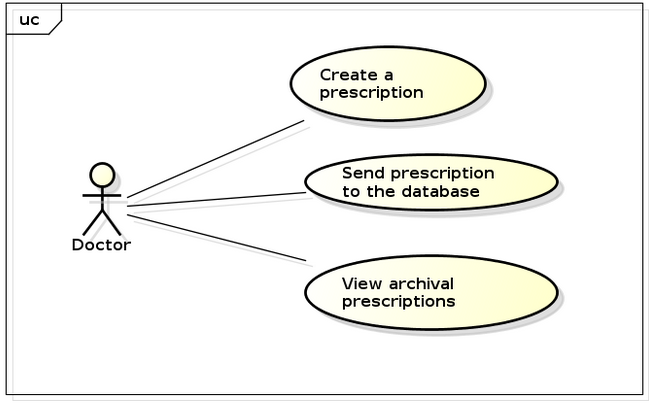
\includegraphics[width=1\textwidth]{doctor/UseCases.png}
\end{figure} 
\textbf{We mark out 3 use cases:}

\begin{itemize}


\item create a prescription - Doctor is generating prescription by collect all needed data and then signature is forged
\item send prescription to the database - prescription sending to database( in some database friendly format)
\item view archival prescriptions - Doctor can check archival prescription of his current patient
\end{itemize}

\subsection{Activity diagram}
It presents system scheme from high level layer and has to show the overall flow of control
\begin{figure}[h]
\centering
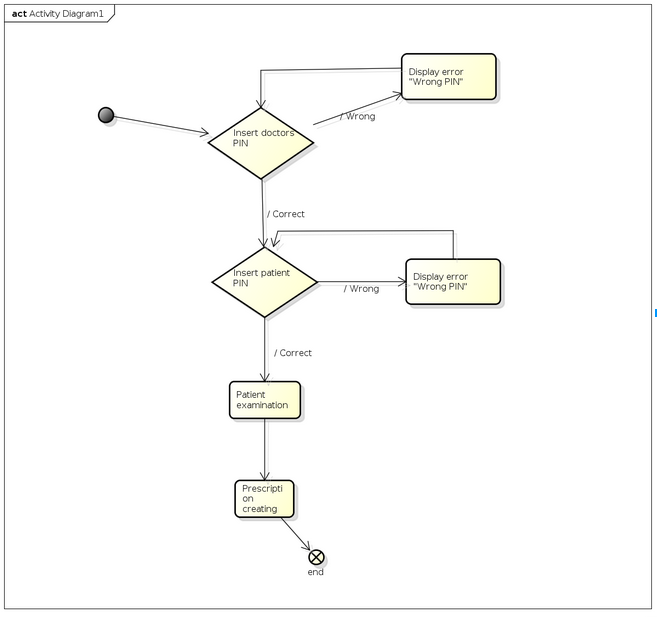
\includegraphics[width=1\textwidth]{doctor/ActivityDiagram.png}
\end{figure} 
\subsection{Sequence diagram}
We present detailed scheme of the system. THe mail goal of this diagram is to present communication between out part, and other parts of the system

%\begin{figure}[h]
%\centering
%\includegraphics[width=\textwidth,height=\textheight,keepaspectratio]%{doctor/WritingOutPrescription2.png}
%\end{figure} 


Writing out a prescription is initialized by the doctor. He can create a prescription on demand or load one previously saved from the csv file. During creation process patients ID should be obtained(from reading patients card or returned by database query). Having newly created prescription, Doctors computer is establishing SSL connection to the database. After this stage, computer requests new value of nonce, by the SQL statement  $getnoncefor(patientid)$.  This nonce and entire prescription should be signed be the doctors card. At the end of the process query to database is made. It should include: nonce, signature over nonce, prescription and signature over prescription.

Database validates both signatures and nonce before inserting any records. Only information inside database can be considered as valid.
%%//Added to there
\subsubsection{View entire patient's history}

%\begin{figure}[p]
%\centering
%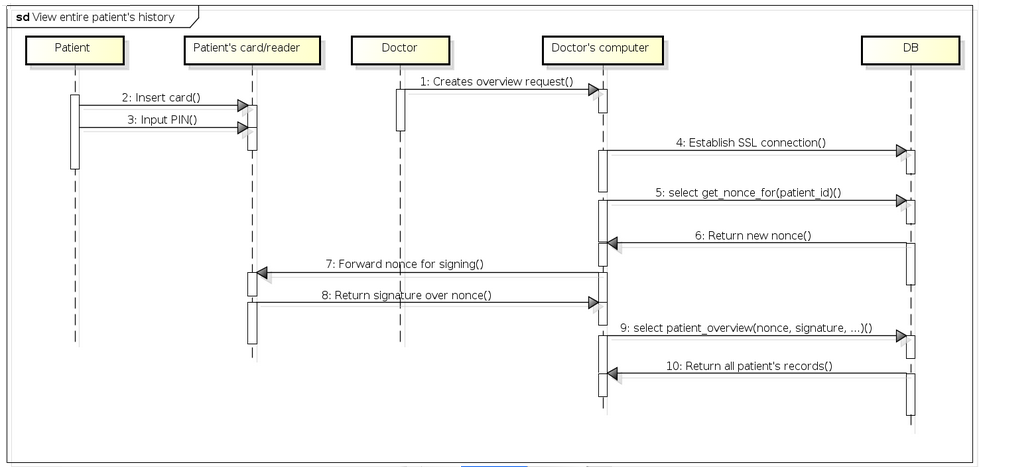
\includegraphics[width=\textwidth,height=\textheight,keepaspectratio]{doctor/HistoryCheckout.png}
%\end{figure} 

View entire patient`s history is initialized by the doctor. First of all, doctor creates overview request. During the process patient`s ID should be obtained(from reading patient`s card or returned by database query). Having the request, Doctor`s computer is establishing SSL connection to the database. After this stage, computer requests new value of nonce, by the SQL statement  $getnoncefor(patientid)$.  This nonce and entire prescription should be signed be the doctor`s card.

At the end of the process query to database is made. It should include: nonce, signature over nonce, request and signature over request.  Database after successful  validation return patient`s records.
\section*{Notes}
There is no need to require doctor`s signature in this procedure. Process requires the presence of a patient and his willingness, so only the owner of the card should be verified. Adding doctor`s signature doesn`t change anything. It only increase computation time and data amount sended across the internet. 

\section{Prescription}
In this part we propose structure of prescription defined using ASN.1. We do not specify format of records in database, it is just a formal specification of object ?Prescription? with information that it has to contain(i.e. it can be even concatenation of all fields specified lower splited by \";\").

\begin{figure}[h]
\centering
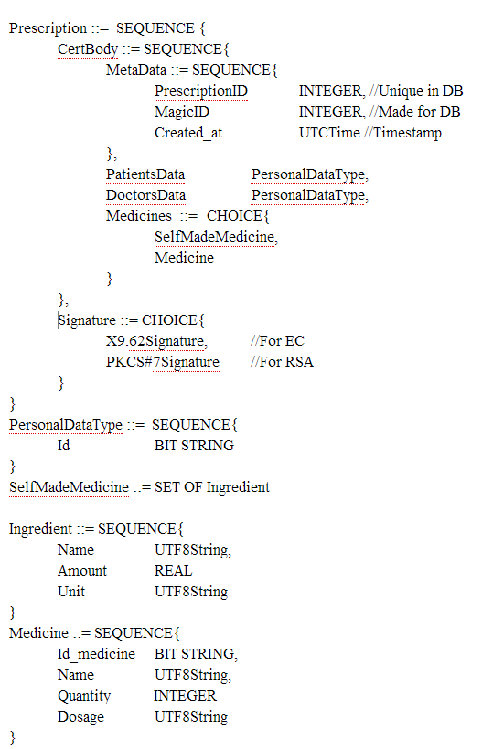
\includegraphics[width=\textwidth,height=\textheight,keepaspectratio]{doctor/asn1.png}
\end{figure} 
In this model it is obvious that pharmacist`s signature is equal to fully realized prescription


\section{Signature}

There is a lot of signature schemes that can be used according to standards (like PKCS\# or X9.63) so we do not specify which should be used yet. We want to mark a situations in protocols that has to be signed.
\subsection{Doctor signature over prescription, and pharmacist signature as a proof that prescription is realized.
}
Prescription as a tuple of data and signature can be signed by doctor and then creating prescription process has been completed. Now when pharmacist is realizing prescription, he has to generate another signature over that tuple with some pharmacist personal data and concat it to prescription. If pharmacist sign prescription, it means that prescription is realized (fully because there is only 1 medicine per prescription)

In this scenario there is still possibility to generate prescription without patient knowledge, but it can not be realized without him, so this sheme is still secure. 

Doctor has to compute signature, because it is a proof that prescription is valid and is signed by specified person. Without it, there is possibility to craft a lot of prescription without knowledge who is trying to spam database.

\subsection{Patient needs to generate signature when patient archival prescription has to be available}

There is a use case, when a doctor wants to look into archival prescription of a patient. Core of a system sends then a nounce (random generated byte`s array) that has to be signed by a patient as a proof that patient allow doctor to check his archival prescription. The Core is not signing a nounce so there is possibility to Adversary (i.e. doctor) to make chosen message attack, so we need to choose digital signature scheme that is unbreakable by chosen-message attack(should we specify what is this?). 

Patient needs to generate signature because he is computing a request that says to DB that he want access to archival prescription. Without it, we do not have a mechanism to confirm this request by patient, so there is opportunity to make request for access without a patient knowledge.

\section{Database integration}
The connection to database is authenticated by Two-way SSL and password. Each party in this process have their own X.509 certificate signed by the CA authority. During authentication process each party verifies certificate of another entity, to be sure that entity is exactly who claims to be. Password is required for specify the username to the database.

Whenever prescription is created by the doctor it has to be send to the database and only the prescription inside database can be valid. Sending process requires to be authenticated and it`s done by the invoke of stored procedure inside database. Procedure takes all information about a prescription at once (specified in section 3).

